%------------------------------------------------------------------------------
% Author(s):
% Varaun Ramgoolie
%
% Copyright:
%  Copyright (C) 2020 Brad Bachu, Arjun Mohammed, Varaun Ramgoolie, Nicholas Sammy
%
%  This file is part of Applied-Mathematics-Unit2 and is distributed under the
%  terms of the MIT License. See the LICENSE file for details.
%
%  Description:
%     Year: 2014
%     Module: 3
%     Question: 6
%------------------------------------------------------------------------------

%------------------------------------------------------------------------------
% 6 a
%------------------------------------------------------------------------------

\begin{subquestions}
	
\subquestion

\textbf{\textit{Simplify and Diagram:}} \\ \\
\begin{figure}[H]
	\begin{center}
		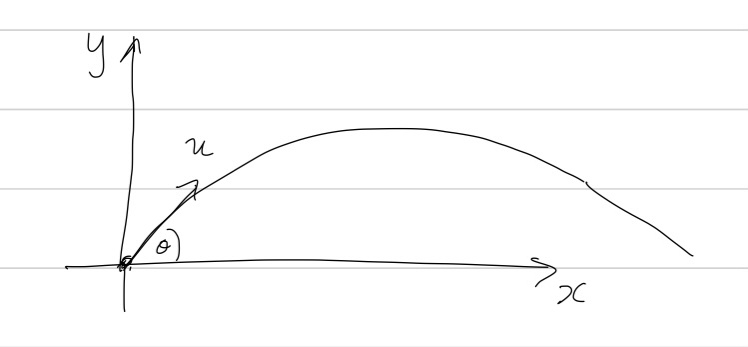
\includegraphics[scale=0.25]{../2014/figures/2014q6-1}
		\caption{\label{2014:q6:Diagram1} Motion of Projectile.}
	\end{center}
\end{figure}
We want to describe the trajectory of a projectile with an equation. We can do this by considering the vertical and horizontal motion of the projectile separately and linking both using the time variable, $t$. We will use,
\begin{itemize}
	\item $\vec{u}$ to represent the initial velocity of the particle,
	\item $\theta$ to represent the angle of projection to the horizontal,
	\item $y$ to represent the vertical displacement of the particle,
	\item $x$ to represent the horizontal displacement of the particle,
	\item $u_x$ to represent the initial velocity of the particle in the horizontal ($x$) direction,
	\item $u_y$ to represent the initial velocity of the particle in the vertical ($y$) direction,
	\item $a_x$ tp represent the acceleration in the $x$ direction,
	\item $a_y$ to represent the acceleration in the $y$ direction,
\end{itemize}  
	
	
	
	
\textbf{\textit{Represent Mathematically:}} \\ \\
Firstly, we should notice that we can resolve $\vec{u}$ as\footnote{We will use the magnitude of $\vec{u}$ as $u$.},
\begin{equation}
	\vec{u} = u\cos(\theta)\xhat + u\sin(\theta)\yhat \,. \label{2014:q6:Eqn1}
\end{equation}

To complete the solution, we will use,
\begin{equation}
	s = ut + \frac{1}{2}at^2 \,.
\end{equation}




\textbf{\textit{Solve and Evaluate:}} \\ \\
From \req{2014:q6:Eqn1}, we get that.
\begin{align}
	u_x & = u\cos(\theta) \\
	& \text{and} \nn \\
	u_y & = u\sin(\theta) \,.
\end{align} 

We will first consider the horizontal motion of the particle. Using $a_x=0$,\footnote{There is no resistance to motion in the $x$ direction, which means that $a_x=0$} $s=x$ and $u_x=u\cos(\theta)$, we get that,
\begin{align}
	s & = ut + \frac{1}{2}at^2 \nn \\
	x & = u\cos(\theta)t + \frac{1}{2}(0)t^2 \nn \\
	\implies t & = \frac{x}{u\cos(\theta)} \nn \\
	           & = \frac{x\sec(\theta)}{u} \,.
\end{align}	

We can now consider the vertical motion of the particle. Using $a_y=-g$,\footnote{The particle's acceleration in the $y$ direction is the acceleration due to gravity. The value is negative as we have taken up to be positive.} $s=y$, $u_y=u\sin(\theta)$ and $t=\frac{x\sec(\theta)}{u}$, we get that,
\begin{align}
	s & = ut + \frac{1}{2}at^2 \nn \\
	y & = u\sin(\theta)\left(\frac{x\sec(\theta)}{u}\right) + \frac{1}{2}(-g)\left(\frac{x\sec(\theta)}{u}\right)^2 \nn \\
	  & = x\tan(\theta) - \frac{gx^2\sec^2(\theta)}{2u^2} \,.
\end{align}
	
%------------------------------------------------------------------------------
% 6 b
%------------------------------------------------------------------------------
	
\subquestion
We are given a situation where a ball is projected at an angle to the horizontal.

\begin{subsubquestions}
	
\subsubquestion

\textbf{\textit{Sketch and Translate:}} \\ \\
\begin{figure}[H]
	\begin{center}
		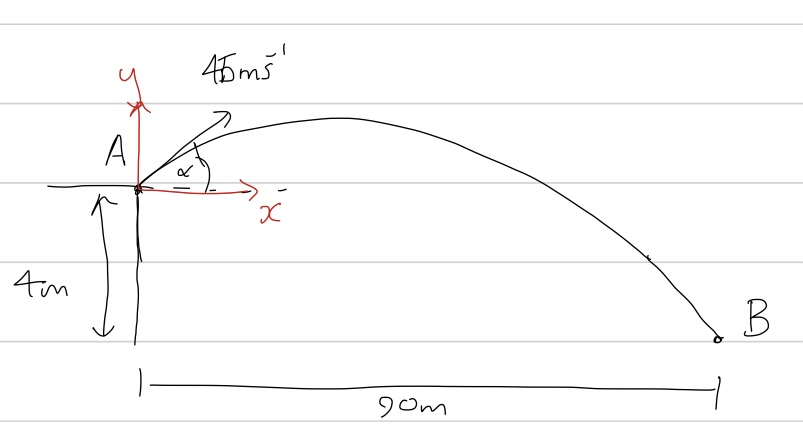
\includegraphics[scale=0.25]{../2014/figures/2014q6-2}
		\caption{\label{2014:q6:Sketch2} Motion of Ball.}
	\end{center}
\end{figure}
From the information given, we can formulate a series of equations and obtain the given expression. We should begin to think about how we can use our equations of motion.




\textbf{\textit{Simplify and Diagram:}} \\ \\
\begin{figure}[H]
	\begin{center}
		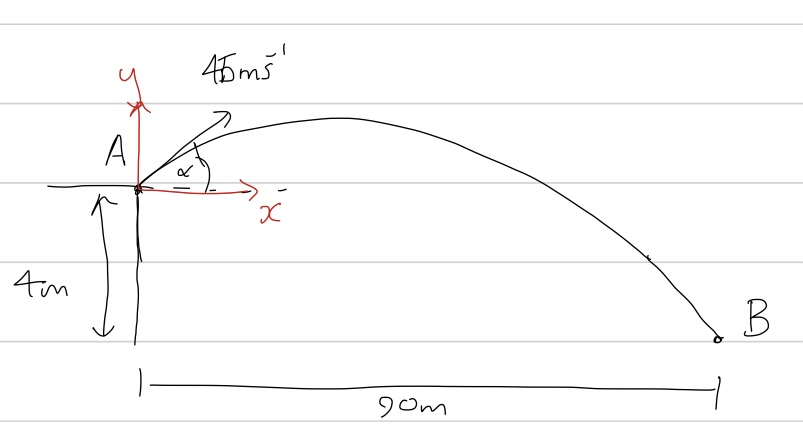
\includegraphics[scale=0.25]{../2014/figures/2014q6-2}
		\caption{\label{2014:q6:Diagram2} Motion of Ball.}
	\end{center}
\end{figure}
We will use,
\begin{itemize}
	\item $u$ to represent the initial velocity of the particle,
	\item $\alpha$ to represent the angle of projection to the horizontal,
	\item $y$ to represent the vertical displacement of the particle,
	\item $x$ to represent the horizontal displacement of the particle,
	\item $u_x$ to represent the initial velocity of the particle in the horizontal ($x$) direction,
	\item $u_y$ to represent the initial velocity of the particle in the vertical ($y$) direction,
	\item $a_x$ tp represent the acceleration in the $x$ direction,
	\item $a_y$ to represent the acceleration in the $y$ direction,
\end{itemize}  




\textbf{\textit{Represent Mathematically:}} \\ \\
At point B, we are given that,
\begin{align}
	x & = 90 \\
	  & \text{and} \nn \\
	y & = -4 \,
\end{align}

From part (a), we know that,
\begin{equation}
	y = x\tan(\alpha) - \frac{gx^2\sec^2(\alpha)}{2u^2} \,.
\end{equation}




\textbf{\textit{Solve and Evaluate:}} \\ \\
By substituting $y=-4$, $x=90$, $u=45$ and $g=10$ at Point B, we get that,
\begin{align}
	-4 & = 90\tan(\alpha) - \frac{10(90)^2\sec^2(\alpha)}{2(45)^2} \nn \\
	-4 & = 90\tan(\alpha) - 20\sec^2(\alpha) \nn \\
	-4 & = 90\tan(\alpha) - 20(\tan^2(\alpha)+1) \nn \\
	16 & = 90\tan(\alpha) - 20\tan^2(\alpha) \nn \\
	&\implies 20\tan^2(\alpha)-90\tan(\alpha)+16 = 0 \,.
\end{align}

%------------------------------------------------------------------------------

\subsubquestion

\textbf{\textit{Simplify and Diagram:}} \\ \\
We can use \rfig{2014:q6:Diagram2}. Our two possible values of $\alpha$ come from solving the quadratic equation in (b)(i).
	
	
	
	
\textbf{\textit{Represent Mathematically:}} \\ \\
We are required to solve,
\begin{equation}
	20\tan^2(\alpha)-90\tan(\alpha)+16 = 0 \,.
\end{equation}
	
	
	
	
\textbf{\textit{Solve and Evaluate:}} \\ \\
By substituting $a=20$, $b=-90$ and $c=16$, we get that,
\begin{align}
	\tan(\alpha) & = \frac{-b \pm \sqrt{b^2-4ac}}{2a} \nn \\
	             & = \frac{90 \pm \sqrt{8100-1280}}{40} \nn \\
	             & = \frac{90 \pm 82.58}{40} \nn \\
	             & = 2.25 \pm 2.06 \,.
\end{align}
	
Our values of $\alpha$ are,
\begin{align}
	\tan(\alpha) & = 4.31 \nn \\
	\implies \alpha & = \arctan(4.31) \nn \\
	                & = 76.94^o \\ \nn \\
	\tan(\alpha) & = 0.19 \nn \\
	\implies \alpha & = \arctan(0.19) \nn \\
					& = 10.76^o \,.
\end{align}
	
%------------------------------------------------------------------------------

\subsubquestion

\textbf{\textit{Simplify and Diagram:}} \\ \\
We can use \rfig{2014:q6:Diagram2}. We can find the minimum time of flight by using our values of $\alpha$ and our equations of motion.




\textbf{\textit{Represent Mathematically:}} \\ \\
By considering our horizontal\footnote{We have considered the horizontal motion as it gives a much more direct solution. We can only do this because we know the horizontal displacement of the particle from point A to point B.} motion at point B, we know that,
\begin{equation}
	x=90 \,.
\end{equation} 

We can find our time of flight using,
\begin{equation}
	x = u_xt + \frac{1}{2}at^2 \,.	
\end{equation}




\textbf{\textit{Solve and Evaluate:}} \\ \\
By substituting $x=90$, $u_x=45\cos(\alpha)$, $a=0$, we get that,
\begin{align}
	90 & = 45\cos(\alpha)t + \frac{1}{2}(0)t^2 \nn \\
	\implies t & = \frac{2}{\cos(\alpha)} \,.
\end{align}

To find our minimum time of flight, we substitute our values of $\alpha$ as,
\begin{align}
	(\alpha=76.94): t & = \frac{2}{\cos(76.94)} \nn \\
	                  & = 8.85 \,. \\
	(\alpha=10.76): t & = \frac{2}{\cos(10.76)} \nn \\
					  & = 2.04 \,. \\	                  
\end{align}

Thus, the minimum time of flight is 2.04s.

\end{subsubquestions}
	
%------------------------------------------------------------------------------
% 6 c
%------------------------------------------------------------------------------

\subquestion

\textbf{\textit{Sketch and Translate:}} \\ \\
\begin{figure}[H]
	\begin{center}
		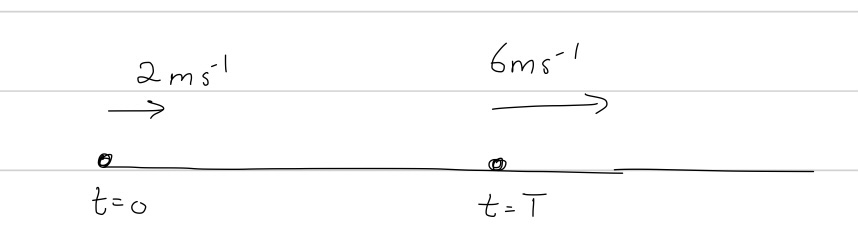
\includegraphics[scale=0.25]{../2014/figures/2014q6-3}
		\caption{\label{2014:q6:Sketch3} Motion of P.}
	\end{center}
\end{figure}
We are given the motion of a particle $P$ on the x-axis with variable acceleration. We should begin thinking about how we use variable acceleration and velocity.




\textbf{\textit{Simplify and Diagram:}} \\ \\
\begin{figure}[H]
	\begin{center}
		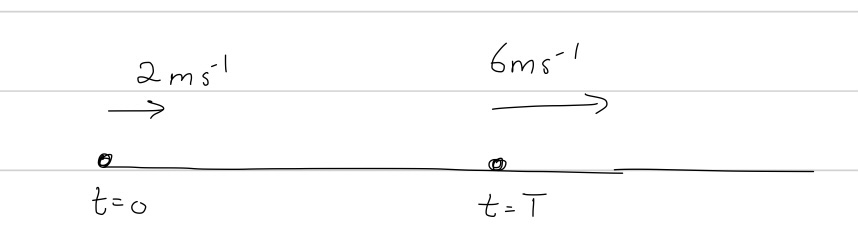
\includegraphics[scale=0.25]{../2014/figures/2014q6-3}
		\caption{\label{2014:q6:Diagram3} Motion of P.}
	\end{center}
\end{figure}
We want to find the find the time $T$ such that the velocity of the particle is 6ms$^{-1}$. As we are given that the acceleration of $P$ is a function of time, we can formulate a differential equation and solve for $T$.




\textbf{\textit{Represent Mathematically:}} \\ \\
By definition, we know that,
\begin{equation}
	a = \ddd{}{t}v \,.
\end{equation}

By the Fundamental Theorem of Calculus, we get that,
\begin{align}
	\int_{t_1}^{t_2}a \dd t & = \int_{v_1}^{v_2} \dd v \nn \\
	\implies \int_{t_1}^{t_2}a \dd t & = v_2-v_1 \,. \label{2014:q6:FTC1}
\end{align}




\textbf{\textit{Solve and Evaluate:}} \\ \\
Substituting $(v_1,t_1)=(2,0)$ and $(v_2,t_2)=(6,T)$ into \req{2014:q6:FTC1}, we get that,
\begin{align}
	\int_{0}^{T} (3t+5) \dd t & = 6-2 \nn \\
	\left[\frac{3t^2}{2} +5t \right]^T_0 & = 4 \nn \\
	\implies \frac{3T^2}{2} +5T & = 4 \nn \\
	3T^2 +10T-8 & = 0 \nn \\
	(3T-2)(T+4) & = 0 \nn \\
	\implies T & = -4,~\frac{2}{3} \,.
\end{align}

Our value of $T$ is $\frac{2}{3}$s as we take the positive value of the time. \TODO{Maybe add graph}

%------------------------------------------------------------------------------
% 6 d
%------------------------------------------------------------------------------

\subquestion

\textbf{\textit{Sketch and Translate:}} \\ \\
\begin{figure}[H]
	\begin{center}
		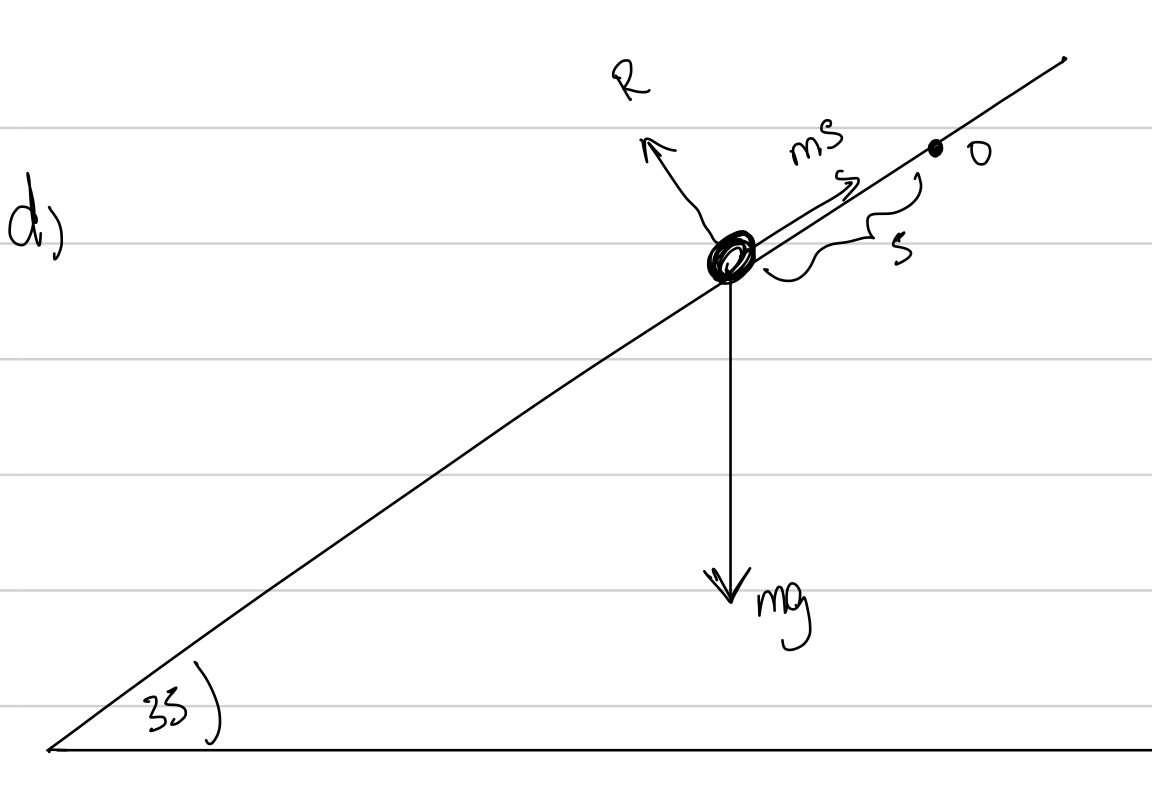
\includegraphics[scale=0.25]{../2014/figures/2014q6-4}
		\caption{\label{2014:q6:Sketch4} Particle sliding down plane.}
	\end{center}
\end{figure}
We are given a particle which slides down an inclined plane with a variable resistive force on the particle.




\textbf{\textit{Simplify and Diagram:}} \\ \\
\begin{figure}[H]
	\begin{center}
		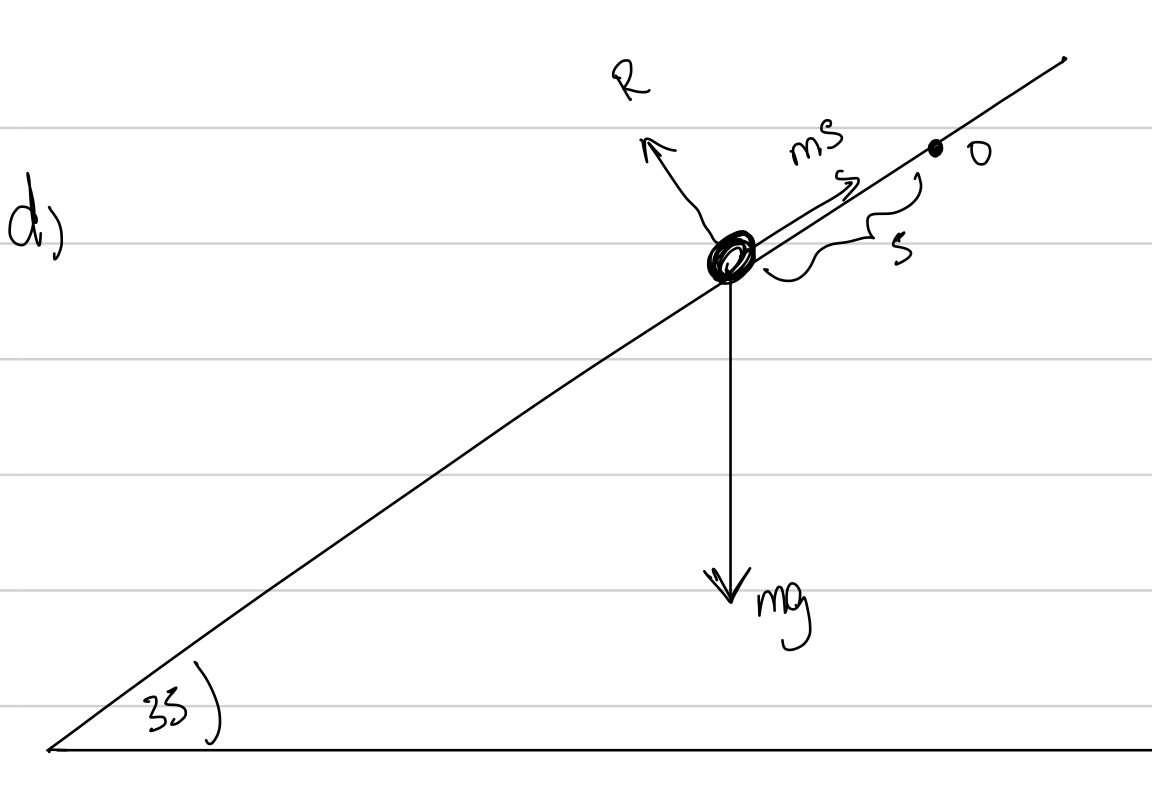
\includegraphics[scale=0.25]{../2014/figures/2014q6-4}
		\caption{\label{2014:q6:Diagram4} Particle moving down plane.}
	\end{center}
\end{figure}
We will first assume that the body behaves as a point particle. Let us represent the forces on the body as,
\begin{itemize}
	\item $W$ which is the weight of the particle,
	\item $F_r$ which is the resistive force on the particle,
	\item $R$ which is the normal reaction force.
\end{itemize}
We will assume that there are no other forces which act on the particle. We will resolve $W$ (parallel and perpendicular to the plane) and use Newton's Second Law to find the variable resultant force on the body. We can then formulate a differential equation and solve.




\textbf{\textit{Represent Mathematically:}} \\ \\
We can resolve $W$ as,
\begin{align}
	\vec{W} & = |W|\sin(35)\xhat - |W|\cos(35)\yhat \nn \\
	        & = mg\sin(35)\xhat - mg\cos(35)\yhat \,.
\end{align}

Using Newton's Second Law, we can find the resultant force, $F_x$, in the $x$ direction as,
\begin{align}
	\sum F \xhat & = mg\sin(35)\xhat - ms\xhat \nn \\
	    F_x & = mg\sin(35) - ms \nn \\
	    \implies ma & = mg\sin(35) - ms \nn \\
	    a & = g\sin(35) - s \,.
\end{align}

Since $s$ is variable, $a$ is also variable and thus,
\begin{align}
	a & = g\sin(35) - s \nn \\
	v\ddd{v}{s} & = g\sin(35) - s \,.
\end{align}




\textbf{\textit{Solve and Evaluate:}} \\ \\
By separating variables, we can obtain the differential equation,
\begin{equation}
	v\dd v = (g\sin(35) - s) \dd s \,.
\end{equation}

By the Fundamental Theorem of Calculus, using $(v_1,s_1)=(0,0)$ and $(v',s_2)=(v',3)$ we get that,
\begin{align}
	\int_{v_1}^{v'}v \dd v & = \int_{s_1}^{s_2} (g\sin(35) - s) \dd s \nn \\
	\int_{0}^{v'}v \dd v & = \int_{0}^{3} (g\sin(35) - s) \dd s \nn \\
	\left[\frac{v^2}{2}\right]^{v'}_0 & = \left[gs\sin(35)-\frac{s^2}{2} \right]^3_0 \nn \\
	 \frac{v'^2}{2} & = 3g\sin(35) - \frac{9}{2} \nn \\
	\implies v'& = \sqrt{6g\sin(35)-9} \nn \\
	           & =  \sqrt{60\sin(35)-9} \nn \\
	           & = 5.04 \text{ms}^{-1} \,.	           
\end{align}

\end{subquestions}